\documentclass[a4paper,12pt]{ctexart}
\usepackage{xeCJK}
\usepackage{booktabs}
\usepackage{enumerate}
\usepackage{graphicx}
\usepackage[normalem]{ulem}
\usepackage{amsmath}
\usepackage{amsfonts}
\usepackage{amssymb}
\usepackage{float}
\usepackage[style=gb7714-2015ay]{biblatex}
\addbibresource{ref.bib}
\usepackage[hidelinks]{hyperref}
\usepackage[table,xcdraw]{xcolor}
\author{董晨阳}
\date{\today}
\title{影响企业实施全面风险管理的因素}
\setcounter{secnumdepth}{0}

\renewcommand{\figurename}{表}
\begin{document}
\maketitle
% \tableofcontents
\clearpage
\section{引言}

企业风险管理是一种系统地识别、评估和控制组织资本和收益的财务、法律、战略和安全风险的过程。它旨在帮助企业在制定和执行战略目标的过程中,有效地应对不确定性以及由此带来的风险和机会,增进创造价值的能力。通过进行企业风险管理,企业可以在符合自身价值观和风险偏好的基础上,采取合适的风险应对策略,如规避、转移、分担或降低风险,从而提高运营效率和效果,减少意外损失和成本,抓住潜在机会,实现企业目标并最大化利益相关者价值。

影响企业开展全面风险管理的因素非常复杂和多样,包括外部环境中的政治经济制度变化、社会文化差异、市场竞争态势等不可控因素,也包括内部环境中的公司治理结构、经营战略选择、组织文化氛围等可控因素。因此,企业需要根据自身的特点和情况,采用适合自己的风险管理方法和流程。本文将对国内外关于企业风险管理的相关研究进行复述和梳理,并对不同的理论观点和实践案例进行分析比较,以期为提高我国企业风险管理水平提供一些参考和启示。

\section{国外相关研究}
\subsection{定性视角:从公司和前人论述中总结特征}
\citet{kleffner2003effect}研究了加拿大公司使用企业风险管理的情况,以及与全面风险管理相关的特征、实施全面风险管理的障碍和公司治理指导方针在决定采用全面风险管理中的作用。这篇文章通过向加拿大风险和保险管理协会成员发送邮件调查并对19名回复者进行电话访谈来收集数据。文章发现,样本中有31\%的公司采用了全面风险管理,采用全面风险管理的原因包括风险经理的影响(61\%)、董事会的鼓励(51\%)和遵守多伦多证券交易所(TSE)指导方针(37\%),而阻碍全面风险管理的因素是不利于全面风险管理的组织结构和总体抗拒变化的态度。其中,上市于TSE与否并没有明显提升全面风险管理的使用。但是37\%的公司表示TSE指导方针在他们决定采用全面风险管理时有影响,这提供了一些证据表明这些指导方针正在影响公司的风险管理策略。

\citet{kleffner2003effect}也有一些局限性和不足之处,例如文章没有深入地分析全面风险管理的影响因素和效果,只是简单地列出了一些相关的变量和统计结果。文章也没有考虑到其他可能影响全面风险管理的因素,比如公司的规模、行业、战略、文化等。

\citet{oliveira2019critical}旨在识别哪些关键成功因素对实施企业风险管理有最大的影响。为了实现这一目标,本研究进行了系统和结构化的文献综述,从而确定了10个全面风险管理倡议的关键成功因素,分别是:(1)管理层的承诺;(2)风险偏好与容忍度;(3)抓住机遇的能力;(4)对全面风险管理的关注度;(5)风险意识和风险文化;(6)资源可获得性;(7)风险识别、分析和响应;(8)风险指标、监测、审查和改进;(9)交流渠道;(10)法律。然后该研究还采用了专家咨询法,通过邀请来自不同行业和领域的93位专家,对文献综述得出的关键成功因素进行验证和补充。本研究最后使用了层次分析法,通过让专家对关键成功因素进行两两比较,计算出每个因素的权重和优先级。
\begin{figure}[H]
    \caption{不同因素的专家得分}
    \centering
    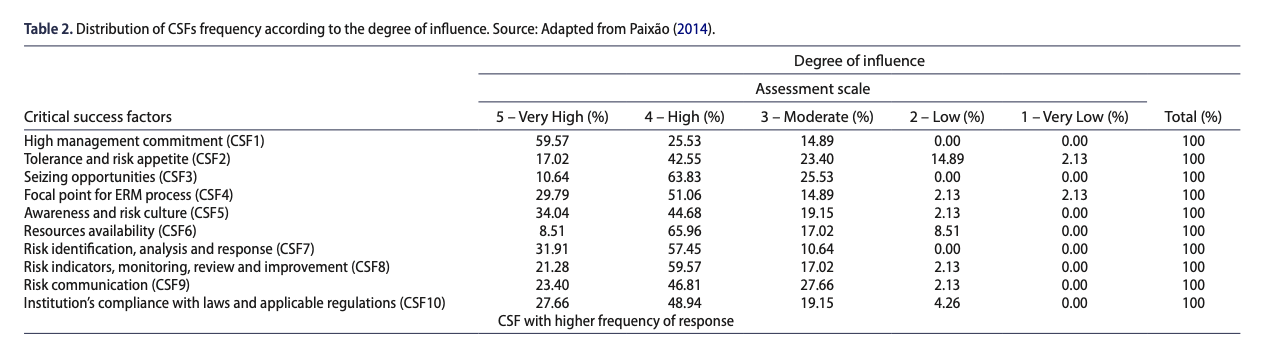
\includegraphics[width=\linewidth]{img/olivia.png}
\end{figure}

\citet{oliveira2019critical}提供了一个全面而系统的框架,用于识别和评估全面风险管理实施过程中的关键成功因素,但也存在一些局限性,比如样本量较小、专家主观性较强、未考虑不同行业和组织的特殊性等。此外,这篇文章的一些假设在现实中可能不成立,从而导致文章结论可能会改变,比如:文章假设全面风险管理是一个统一且标准化的过程,但实际上不同组织可能有不同的全面风险管理模型和方法。文章假设全面风险管理是一个技术性且客观性的过程,但实际上全面风险管理涉及到人力、社会、政治、伦理等多方面的因素。

\citet{jean2021rethinking}认为全面风险管理是一种能够让组织更具前瞻性和有效性地评估、接受和管理各种风险的风险管理方法,但是很多组织在实施全面风险管理的过程中遇到了挫折和困难。文章提出了一个理论框架,从社会因素(组织结构、角色、人类行为和组织内部工作质量等)和技术因素(组织工作系统中的技术、政策、规则、程序和相关知识等)两个方面,分析了影响全面风险管理成功实施的关键因素。文章还借鉴了社会技术理论、互适应理论和动态能力理论,来构建全面风险管理实施的概念化模型。

\citet{jean2021rethinking}文章的优点是提出了一个新颖且有启发性的视角来看待全面风险管理实施的问题,强调了社会技术因素在全面风险管理实施中的重要性,扩展了全面风险管理的理解范围,将全面风险管理与管理实践的挑战联系起来。文章也借用了三个理论视角来增强其框架的可信度和适用性。文章的缺点是没有进行实证研究或案例分析来检验其框架或假设,也没有提供具体的操作性建议或指导来帮助组织实施全面风险管理。文章也没有充分考虑全面风险管理实施过程中可能存在的环境变化、不确定性、复杂性和动态性等因素,也没有讨论全面风险管理实施对组织绩效或价值的影响或衡量方式。我个人比较赞同文章的结论,即全面风险管理实施需要考虑社会技术因素,并且需要有动态能力来适应变化。
\subsection{定量视角:对总结因素进行回归分析}
\citet{beasley2005enterprise}根据文献及COSO标准梳理出影响企业实施企业风险管理的因素,包括组织结构、治理机制、审计特征、规模和行业等。文章运用多元回归分析,发现全面风险管理实施程度与首席风险官的存在、董事会独立性、CEO和CFO对全面风险管理的支持、四大会计师事务所的审计、组织规模以及银行、教育和保险行业有正相关关系,而与美国组织有负相关关系。

文章采用了定量研究的方法,利用问卷调查收集了123个组织的数据,包括全面风险管理实施程度、组织结构、治理机制、审计特征、规模和行业等变量。文章使用了多元回归分析来检验全面风险管理实施程度与其他变量之间的关系,控制了一些可能的混杂因素,如地区、年份等。文章还进行了敏感性分析和稳健性检验,以验证结果的可靠性。
\begin{figure}[H]
    \caption{Logit多元回归的结果显著}
    \centering
    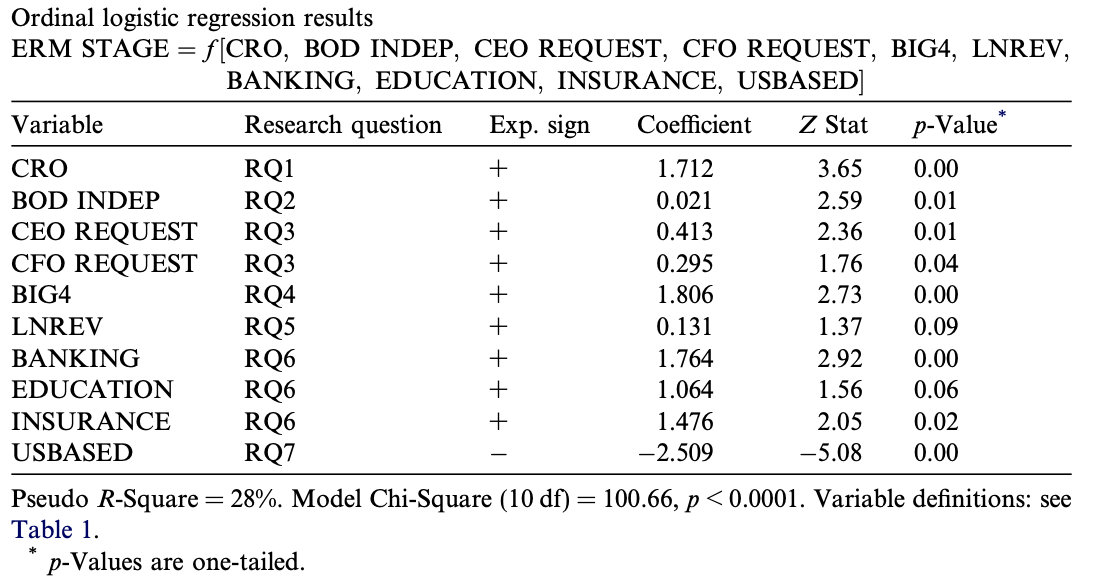
\includegraphics[width=\linewidth]{img/logits.png}
\end{figure}

上图中CRO的正向显著系数表明,首席风险官的存在与全面风险管理部署的程度呈正相关。同样,更独立的董事会,以及首席执行官和首席财务官明确要求内部审计参与企业风险管理,也与企业̃部署企业风险管理的程度密切相关。总体而言,这些结果表明,董事会和高级管理层对机构风险管理的态度对机构风险管理的实施至关重要。其他公司特征也与机构风险管理部署的范围有关。与规模较小的公司或非四大会计师事务所审计的企业相比,规模较大且由四大会计师事务所审计的企业更有可能进一步实施企业风险管理。同样,银行、教育和保险行业的公司正在更深入地实施ERM,这可能是因为行业监管机构或领导者明确要求更有效的风险管理。最后,美国公司在(当时)全面风险管理实施方面没有那么先进。

\citet{beasley2005enterprise}为理解全面风险管理的实施情况和影响因素提供了一些有用的见解,也为后续的更深入的研究奠定了基础。文章的不足之处是样本量较小,可能存在选择偏倚或代表性不足的问题,数据来源于自我报告,可能存在测量误差或主观偏差的问题,变量之间的关系可能存在内生性或逆向因果性的问题,以及缺乏对全面风险管理实施效果或绩效影响的评估。我基本赞同文章的结论,但也认为在现实中可能存在一些影响全面风险管理实施效果或绩效影响的因素,如组织文化、风险态度、市场环境、竞争压力等,这些因素可能导致文章的结论在不同情境下有所变化或修正。



\citet{mensah2015enterprise}探讨了企业风险管理(ERM)的实施与三个因素的关系:首席风险官(CRO)的角色、审计委员会(AC)的存在和高层管理者(TM)的支持。文章采用了非实验性的相关性研究方法,通过调查问卷收集了来自风险管理专业人士的数据,使用了多元回归分析来检验ERM实施水平与CRO、AC和TM之间的关系,以及CRO、AC和TM之间的相关性。这篇文章所用的模型如下:
$$ERM = \beta_0 + \beta_1 CRO + \beta_2 AC + \beta_3 TM + \epsilon$$

这篇文章使用了皮尔逊相关系数来度量CRO、AC和TM之间的相关性,发现CRO、AC和TM都与ERM实施水平有显著正相关,即这三个因素都能促进ERM的有效实施;TM与CRO和AC都有显著正相关,即高层管理者的支持能增强首席风险官和审计委员会的作用;此外,CRO和AC之间有较强的正相关,即首席风险官和审计委员会能相互协调和配合。

\citet{lackovic2022three}探索企业风险管理在非金融公司中的实施情况,以及是否与COSO ERM框架有差异。通过文献综述,提出了一些重要的ERM特征,并通过问卷调查的方式,收集了欧洲非金融公司的数据,然后使用探索性因子分析(EFA)对数据进行了统计分析

文章所用的模型是基于三个因子的ERM实施模型,分别是战略、运营和监督。文章首先提取出前人文章的29个因子,使用了主成分分析和方差最大旋转法(varimax rotation)来进一步提取因子,并用Kaiser criterion和scree test来确定因子个数。文章发现了三个显著的因子,分别解释了数据变异的65.16\%、6.77\%和4.85\%,总共解释了76.78\%,文章还使用了因子得分回归法(factor score regression method)来检验因子与原变量的关系,认为这三个因子分别指向了战略、运营和监督三个层面。
\begin{figure}[H]
    \caption{前三主成分经过varimax rotation之后与原变量的关系(部分)}
    \centering
    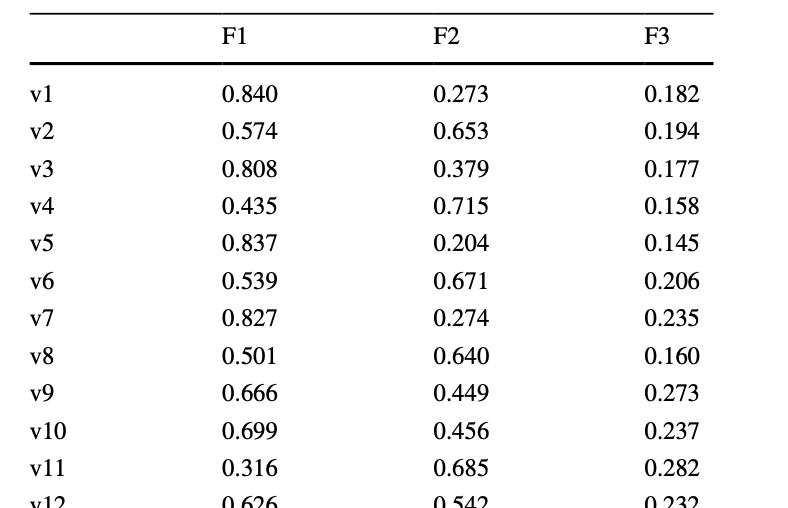
\includegraphics[width=0.6\linewidth]{img/pca.png}
\end{figure}

我认为这篇文章的结论是有道理的,因为它反映了ERM在实践中的复杂性和多样性,以及与COSO ERM框架之间的差距。但这篇文章的一个假设是,问卷调查能够有效地反映公司的ERM实施情况,但是在现实中,可能存在一些偏差或误差,比如回答者的主观性、问卷设计的不完善、样本选择的不代表性等。并且这篇文章只关注了非金融公司,并且只收集了欧洲公司的数据,因此不能推广到其他行业或地区。
\section{国内相关研究}
\subsection{通用行业领域}
\citet{王永海2011全面风险管理成功因素分析}分析了全面风险管理的成功因素,特别是有效激励的作用。文章认为,全面风险管理需要企业全员的参与和协作,但存在一些内生性因素阻碍了这一过程,如信息不对称、代理问题、风险偏好差异等。因此,文章提出了构建有效激励机制的方法,以促进全面风险管理的实施和效果。文章首先通过文献综述,梳理了全面风险管理的概念、特征、目标和影响因素,并指出了有效激励在其中的重要性。然后,文章通过两个案例分析,分别是美国安然公司和中国中石油公司,展示了有效激励在全面风险管理中的具体应用和效果。没有使用数学或统计模型,而是使用了一个逻辑框架来分析全面风险管理的成功因素。文章认为,有效激励的核心是使企业全员的利益与企业整体利益保持一致,并根据不同阶段和不同层级的员工提供相应的奖惩机制。

这篇文章从一个新颖且实用的角度分析了全面风险管理的成功因素,即有效激励。文章结合理论和实证,系统地讨论了有效激励在全面风险管理各个阶段中的作用和方法,并给出文章给出了一些具体的案例和建议,对于企业实施全面风险管理有一定的指导意义。文章的结论也比较符合实际情况,即有效激励是全面风险管理的重要保障。不过,文章也有一些不足之处,例如:文章没有充分考虑有效激励的成本和效益,以及如何平衡不同利益相关者的诉求和期望。例如,设立风险奖金、控制成本预算等措施可能会增加企业的财务负担,而且可能会引起员工之间的竞争和不公平感。文章没有深入分析有效激励的适用范围和条件,以及如何根据不同的风险类型和特征进行差异化的激励设计。例如,对于一些不可预测、不可控制、不可量化的风险,单纯依靠激励机制可能无法有效地识别、评估、控制和监督。文章没有充分考虑有效激励的动态性和可持续性,以及如何根据企业内外部环境的变化进行及时的调整和更新。例如,随着员工的风险意识、能力、偏好等因素的变化,以及市场竞争、监管政策、社会舆论等因素的影响,原有的激励机制可能会失效或适得其反。

\citet{刘红霞2013中国企业实施全面风险管理}则探讨了影响中国企业实施全面风险管理(ERM)的关键因素,以及ERM对企业绩效的影响。文章的研究方法是基于2009年至2011年中国上市公司的数据,运用多元回归等实证方法进行分析。文章的回归结果显示,审计事务所类型、企业规模、财务状况等因素对ERM实施有非常重要的影响;在两职合一的公司治理机制下,管理者权利过于集中,不利于ERM的有效实施;ERM对企业绩效有正向影响,但并不显著。
\begin{figure}[H]
    \caption{回归结果}
    \centering
    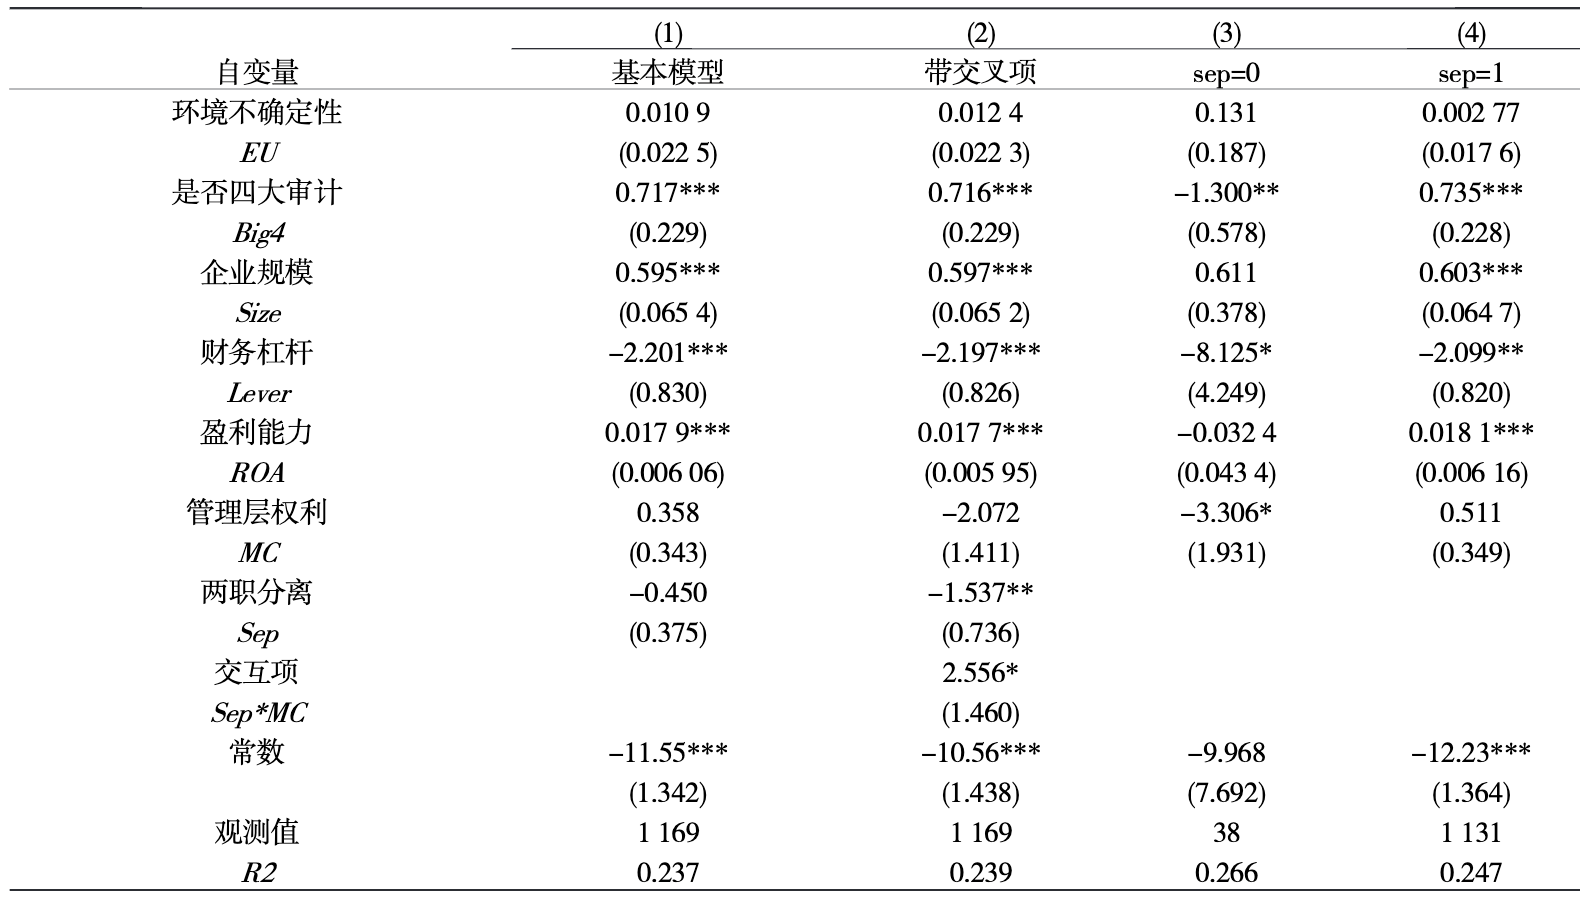
\includegraphics[width=\linewidth]{img/sep.png}
\end{figure}

但是,文章没有考虑到其他可能影响企业绩效的因素,如市场环境、竞争策略、创新能力等,可能导致回归结果存在遗漏变量偏误,文章没有对ERM与企业绩效之间的因果关系进行深入探讨,只是简单地假设ERM对企业绩效有正向影响,忽略了可能存在的反向影响或双向影响。因此,我不完全赞同文章的结论。我认为文章需要进一步完善ERM的定义和测量方法,增加更多控制变量和灵敏度分析,以及运用更多工具变量或面板数据等方法来检验ERM与企业绩效之间的因果关系。

\citet{沈烈2022内部控制对企业风险管理的影响}则回顾了内部控制对企业风险管理影响的理论与应用研究,分析了内部控制与企业风险管理的关系,以及内部控制对系统风险和非系统风险的影响,并展望了未来的研究方向和挑战。文章没有使用具体的数学或统计模型,而是基于COSO内部控制框架和COSO ERM框架,构建了一个概念性的分析框架,将内部控制、企业风险管理、系统风险和非系统风险作为四个关键变量,分析了它们之间的相互作用和影响机制。这篇文章是一篇综述性的文章,没有提供新的实证数据或证据,而是基于现有的文献进行了归纳和总结。文章的优点是涵盖了较多的相关文献,对内部控制与企业风险管理的关系进行了较为全面和深入的分析,提出了一些有价值的观点和建议。文章的不足是缺乏对系统风险和非系统风险的具体度量和划分,没有考虑不同行业、不同规模、不同所有制等因素对内部控制与企业风险管理的影响,也没有对未来可能出现的新型风险进行预测和应对。

我基本赞同文章的结论,即内部控制是企业风险管理的重要组成部分,高质量的内部控制能够有效降低企业的风险,但同时也需要注意内部控制与企业风险管理之间存在动态平衡和协调问题。文章的一些假设在现实中可能不成立,例如假设内部控制与企业风险管理之间存在线性关系,而忽略了可能存在的非线性或阈值效应;假设内部控制与企业风险管理之间存在单向因果关系,而忽略了可能存在的双向反馈或循环作用;假设内部控制与企业风险管理之间存在稳定关系,而忽略了可能存在的时变或异质性效应等。这些假设如果不成立,可能会导致文章结论需要修正或补充。
\subsection{专业行业领域}
\citet{zhao2013critical}的目的是识别和分析中国建筑类公司(这些公司)实施企业风险管理的关键成功因素(CSFs),并提出一个适用于这些公司的ERM框架。这篇文章采用了综合文献回顾和问卷调查的方法,通过对89份有效问卷的因子分析和结构方程模型(SEM)分析,确定了16个关键成功因素,并将它们分为三个潜在的因素群:执行与整合、沟通与理解、以及高层管理的承诺与参与。
\begin{figure}[H]
    \caption{适用于这些企业的关键成功因素}
    \centering
    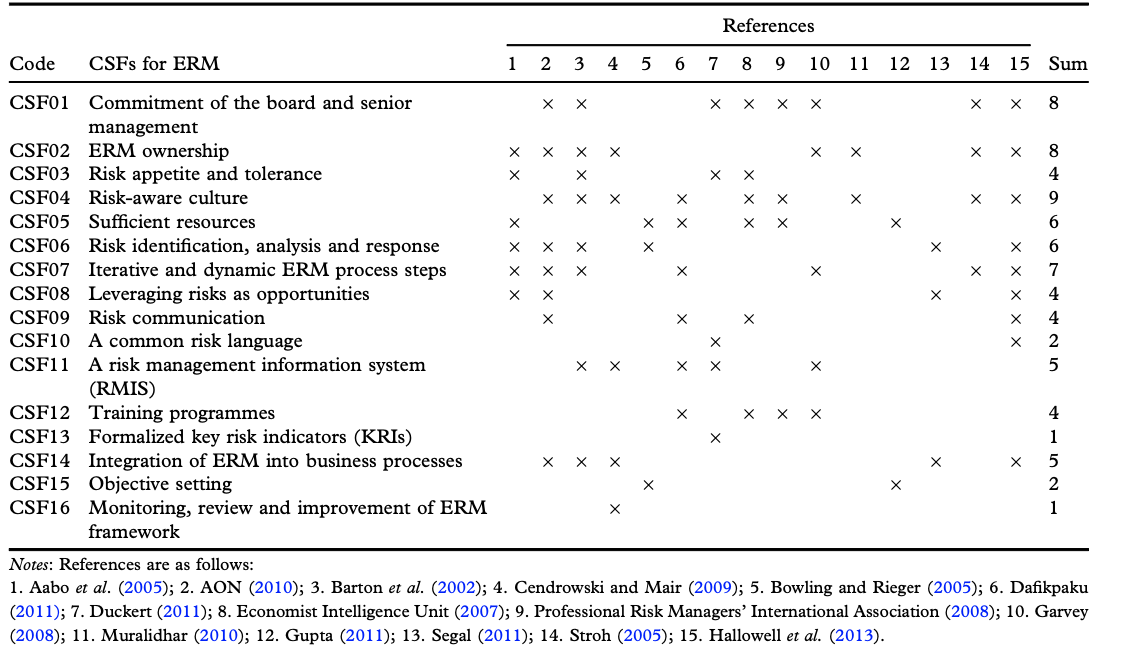
\includegraphics[width=\linewidth]{img/csf.png}
\end{figure}

这篇文章所用的模型是基于SEM的偏最小二乘法(PLS),它可以处理小样本和非正态数据的问题。文章得到了各个关键成功因素之间的路径系数和显著性水平。文章发现,高层管理的承诺与参与对沟通与理解以及执行与整合有正向影响,而沟通与理解也对执行与整合有正向影响。文章还发现,执行与整合对ERM绩效有最大的影响,其次是高管的承诺与参与,最后是沟通与理解。
\begin{figure}[H]
    \caption{不同因素的重要程度}
    \centering
    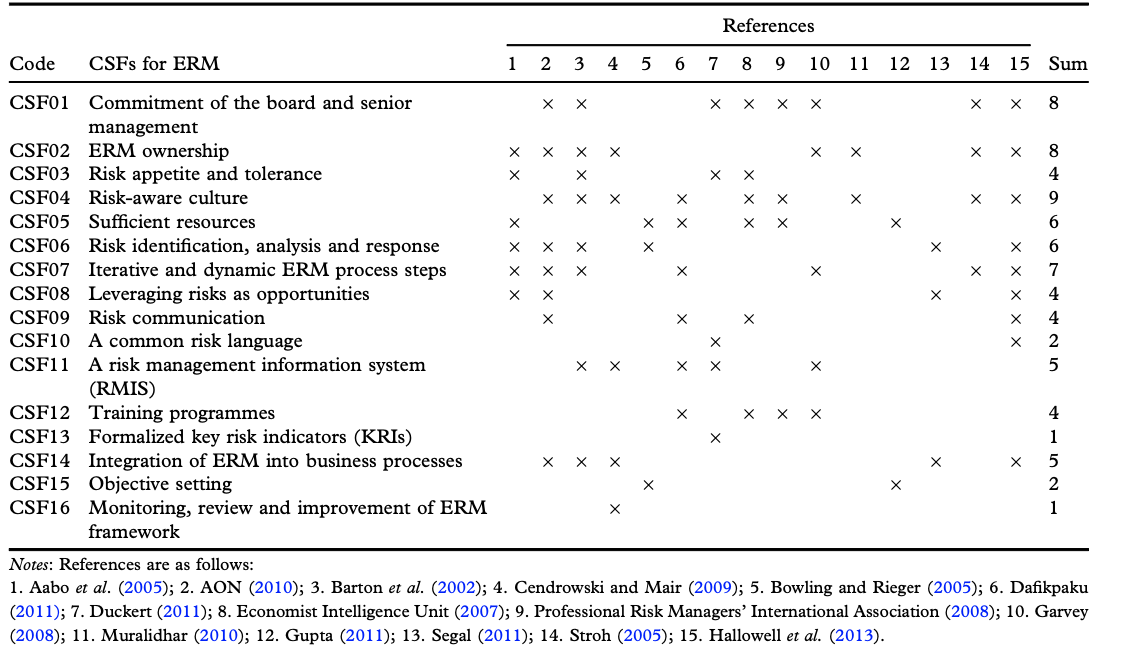
\includegraphics[width=0.6\linewidth]{img/csf.png}
\end{figure}

文章针对了一个重要且具有实践意义的话题,即如何在中国建筑行业实施有效的ERM。文章通过广泛的文献回顾和实证研究,提出了一个适用于这些公司的ERM框架,并揭示了各个关键成功因素之间的相互作用关系。文章也提供了一些对于ERM实施者和研究者有用的建议和启示。但文章也存在一些局限性和不足之处,例如:文章没有考虑不同类型或规模的这些公司可能存在的差异性和多样性,也没有考虑不同地区或市场环境对于ERM实施的影响。文章也没有对ERM绩效进行具体或量化的测量,而是使用了一个单一的潜变量来代表ERM绩效,这可能忽略了ERM绩效的多维性和复杂性。文章也没有对关键成功因素进行优先级排序或权重分配,而是将它们视为同等重要,这可能不符合实际情况。

因此,我认为这篇文章虽然有一定的价值和贡献,但也需要在未来进一步完善和改进。我不完全赞同文章的结论,因为我认为在现实中可能存在一些假设不成立或条件变化的情况,从而导致文章结论可能会改变。例如:如果高层管理缺乏ERM知识或经验,或者对ERM持有错误或偏见的观念,那么他们可能无法有效地承担ERM领导者或推动者的角色,从而影响ERM实施的质量和效果。如果这些公司面临着激烈或不稳定的竞争环境,或者受到外部因素如政策、法律、市场等的影响,那么他们可能需要调整或更新他们的ERM目标或策略,以适应变化的情况。这样的话,文章提出的ERM框架可能就不够灵活或适应性强。

\citet{周运涛2011全面风险管理的影响因素研究}是一篇探讨ERM对中国保险业绩效影响的实证研究。文章采用了问卷调查和多元回归分析的方法,构建了ERM指数和绩效指标,并检验了ERM与绩效之间以及ERM与公司治理、市场竞争、监管环境等变量之间的关系。文章的主要结论是:在中国保险业中,ERM与ROA和ROE呈正相关关系;公司治理水平、市场竞争程度和监管环境对ERM的实施有显著影响。文章的贡献在于,它是国内较早对ERM进行量化测度并分析其影响因素和效果的研究,为中国保险业实施ERM提供了一定的理论依据和实践参考。文章的不足之处在于,它在构建模型时,隐含了一些假设,其中一些在现实中可能不成立或不完全成立。例如:文章假设ERM指数能够充分反映保险公司的风险管理水平,但是该指数是基于问卷调查结果构建的,可能存在主观性和偏差。此外,该指数只考虑了四个维度,可能忽略了其他重要的风险管理方面,如风险文化、风险沟通、风险报告等。文章假设绩效指标能够充分反映保险公司的经营状况,但是这些指标都是基于财务数据计算的,可能忽略了保险公司的非财务方面,如客户满意度、品牌形象、社会责任等。文章假设ERM与绩效之间的关系是单向的,即ERM影响绩效,而不考虑绩效对ERM的反馈作用。但是在实际中,保险公司的经营状况可能会影响其对风险管理的投入和重视程度,从而影响ERM的实施水平。例如,当保险公司盈利能力较强时,可能会增加风险管理的投入和创新,从而提高ERM水平;反之,当保险公司盈利能力较弱时,可能会削减风险管理的投入和创新,从而降低ERM水平。
\section{结论}
本文从全面风险管理的概念、内涵和框架出发,对影响企业实施全面风险管理的因素进行了分析和探讨。通过对国内外相关文献的梳理和综合,本文认为影响企业实施全面风险管理的因素主要有以下几个方面:

一是外部环境因素,包括政治、法律、社会文化、技术和市场等方面的变化和不确定性,给企业经营带来了各种风险和机遇,要求企业及时调整战略和应对措施,提高风险意识和风险管理能力。

二是内部组织因素,包括企业的治理结构、组织架构、人力资源、社会责任、信息系统等方面的建设和完善,影响着企业风险管理的效率和效果,需要企业建立健全风险管理组织保障、体系保障和实施程序。

三是技术创新因素,包括技术设计、研发、应用等方面的风险识别、分析、评估和应对,涉及到技术创新的可行性、有效性和安全性,需要企业充分利用科技手段,提高技术创新的水平和质量。

四是学术研究因素,包括风险管理理论、方法、模型等方面的创新和发展,为企业实施全面风险管理提供了理论指导和工具支持,需要企业关注学术前沿,借鉴国内外先进经验。

综上所述,影响企业实施全面风险管理的因素是多方面的,也是动态变化的。企业要根据自身的特点和发展阶段,结合外部环境的变化趋势,制定适合自己的全面风险管理策略,并持续改进和优化。同时,也要加强与政府、行业协会、学术机构等相关方的沟通和合作,共同推动全面风险管理在我国企业中的普及和提升。

\appendix
\nocite{*}
\printbibliography
\end{document}
